Uma solução saturada de nitrato de potássio (\chemfig{KNO_3}) constituída, além do sal, por \SI{100}{\gram} de água, está à temperatura de \SI{70}{\celsius}.
Essa solução é resfriada a \SI{40}{\celsius}, ocorrendo precipitação de parte do sal dissolvido.
Com base nesses dados e no gráfico apresentado abaixo:

\begin{center}
	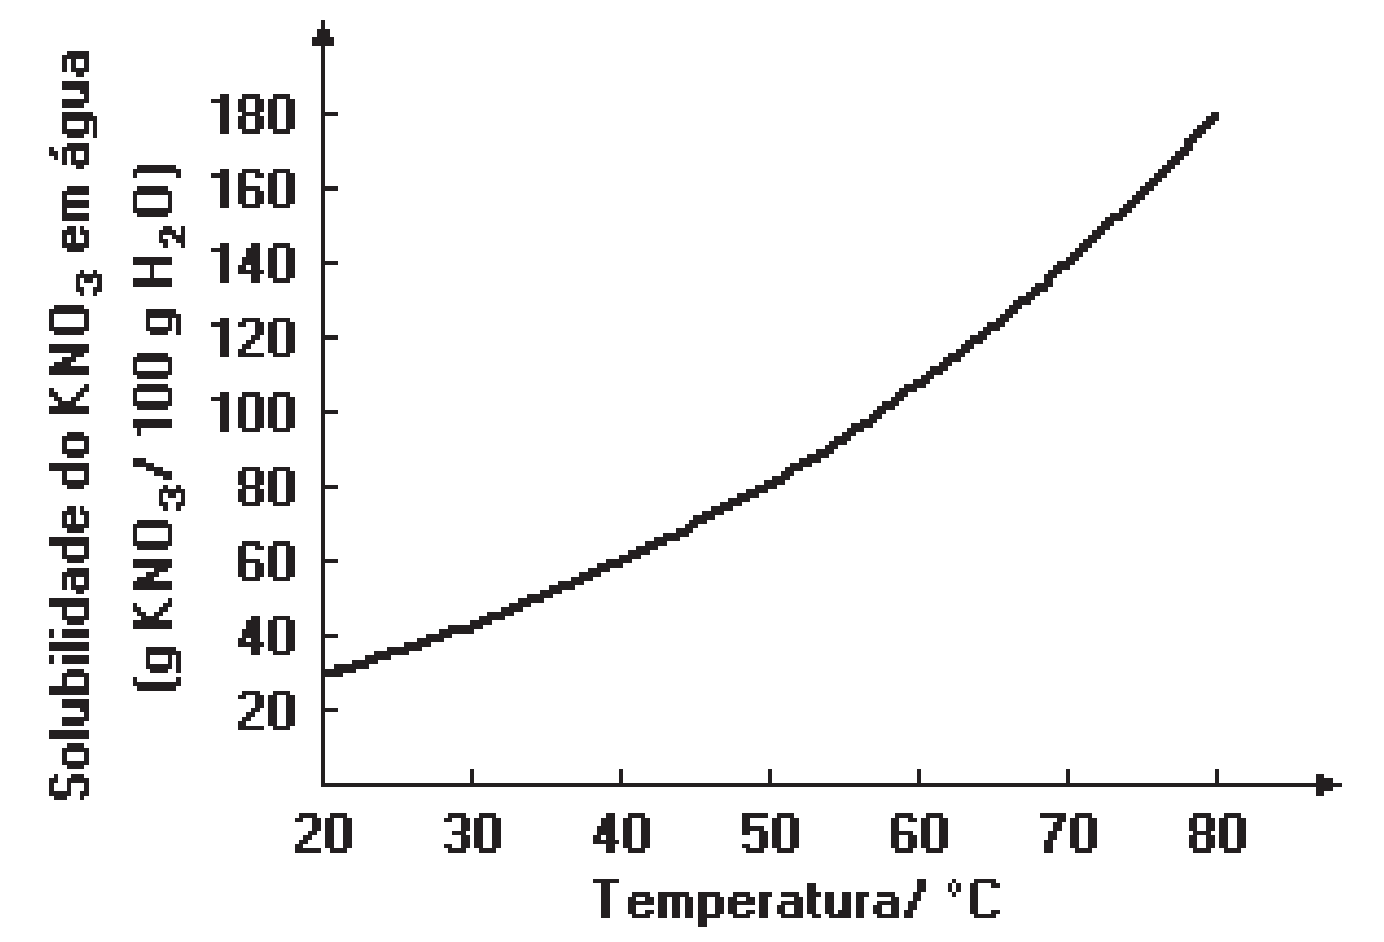
\includegraphics[width = 7cm]{figure.png}
\end{center}

Pode-se afirmar que a massa de sal que precipitou foi de aproximadamente:

\begin{enumerate}[label = (\scalealph{\alph*})]
	\item \SI{20}{\gram}
	\item \SI{40}{\gram}
	\item \SI{60}{\gram}
	\item \SI{80}{\gram}
	\item \SI{100}{\gram}
\end{enumerate}
